\documentclass[12pt]{article}
\usepackage[utf8]{inputenc}
\usepackage{amsmath, amssymb, physics, graphicx, tikz}
\usepackage[a4paper, margin=1in]{geometry}
\usepackage{fancyhdr}
\usepackage{hyperref}
\usepackage{tikz}
\usepackage{xcolor}
\definecolor{sectionrectanglecolor}{rgb}{0.25,0.5,0.75}
\definecolor{sectiontitlecolor}{rgb}{0.2,0.4,0.65}
\definecolor{subsectioncolor}{rgb}{0,0,0}
\definecolor{lightgray}{gray}{0.9}
\definecolor{darkgray}{gray}{0.1}
\definecolor{lightred}{rgb}{0.9,0,0.1}
\usepackage{wrapfig}
\usepackage{tcolorbox}

\newcommand{\be}{\begin{eqnarray}}
\newcommand{\non}{\nonumber \\ }
\newcommand{\ee}{\end{eqnarray}}
\newif\ifshowboardanswers
\showboardanswersfalse
% Set this to \showboardquestiontrue to include the end-of-lecture board question.
\newif\ifshowboardquestion
\showboardquestionfalse
\newcommand{\boardanswer}[1]{\ifshowboardanswers\\[0.35em]\textcolor{blue}{\textbf{Answer.} #1}\fi}

\fancyhead[L]{Special Relativity}
\fancyhead[R]{Lecture 11}

\title{\textbf{Lecture 11: Collisions, Decays, and Particle Physics Units}}
\author{Based on Morin's \textit{Introduction to Classical Mechanics}, Ch. 12.3--12.4}
\date{}

\begin{document}
\maketitle

\section*{Outline}
\begin{enumerate}
    \item \href{sec:recap}{Recap lecture 10}
    \item \href{sec:CandD}{Collisions and Decays}
    \item \href{sec:PPU}{Particle Physics Units.}
\end{enumerate}

\section{Recap lecture 10}\label{sec:recap}

In lecture 10 we heuristically introduced relativistic energy and momentum (in SR units): 
\begin{tcolorbox}[colback=blue!5!white]
\vspace{-1.3em}
\be
{\bf p} = \gamma m{\bf v}, \;\;\;\; E = \gamma m.
\ee
\end{tcolorbox}
Using the limit $v\ll 1$, we found that 
\be
E = m + \frac{1}{2}mv^2
\ee
which allowed us to define kinetic energy as 
\be
E_k = \gamma m - m. 
\ee
Furthermore, 
\begin{tcolorbox}[colback=blue!5!white]
\vspace{-1.3em}
\be
E^2 = |{\bf p}|^2+ m^2. \label{eq:Epm}
\ee
\end{tcolorbox}
and 
\begin{tcolorbox}[colback=blue!5!white]
\vspace{-1.3em}
\be
\frac{\bf p}{E} = {\bf v}.
\ee
\end{tcolorbox}
For a photon, the massive-particle expressions ${\bf p}=\gamma m{\bf v}$ and $E=\gamma m$ are not directly useful because $m=0$ and $v=1$. However, Eq.~\eqref{eq:Epm} gives $E^2=|{\bf p}|^2$ for any massless particle. The energy of a photon is also $E=h\nu$, where $h$ is Planck's constant and $\nu$ is the photon's frequency.


\section{Collisions and Decays}\label{sec:CandD}

Now that we have the expressions for relativistic momentum and energy, we can take a look at collisions and decays.  The approach is the same as before, we simply keep track of all conservation rules, in this case of relativistic energy (1-component) and relativistic momentum (up to 3 components). It is useful to define these components in one vector, the energy-momentum 4-vector, defined as 
\be
P \equiv (E, {\bf p}) = (E,p_x, p_y, p_z).
\ee
We will adopt Morin and use upper-case $P$ for the energy-momentum 4-vector and lower-case ${\bf p}$ for the momentum vector. We will use index notation running from $0$ to $3$, i.e., $P_0 = E$ and $P_i = (p_x, p_y, p_z)$, with $i=1,2,3$. For a single massive particle, we would have $P=(\gamma m,\gamma mv_x, \gamma m v_y, \gamma m v_z)$. For a massless particle moving in the $x$ direction, we would have $P=(E,E,0,0)$. 

Energy and momentum conservation before an interaction of a system would thus be written as 
\be
P_{\rm before} = P_{\rm after},
\ee
where we equate the sum of all particles involved in the interaction, both before and after. 

We can also define an inner product:
\be
A\cdot B = A_0 B_0 - A_1 B_1 - A_2 B_2 -A_3 B_3. 
\ee
Note that we have introduced a minus sign here (which is a relic of Minkowski space). In the next chapter it will become clear why this appears, but it it perhaps already helpful to realize that we can write $\Delta s = (\Delta t, \Delta x, \Delta y, \Delta z)$ as the interval 4-vector, and then realizing that the interval squared $\Delta s^2 = \Delta s \cdot \Delta s$ requires an inner product such as the above to obtain $\Delta s^2 = \Delta t^2 - \Delta x^2 - \Delta y^2 - \Delta z^2$. This inner product is Lorentz invariant, just as the usual 3D inner product is invariant under rotations. 

The inner product defined above also allows us to write:
\be
P \cdot P = E^2 - |{\bf p}|^2 = m^2,
\ee
i.e., $P^2 = m^2$. Note that this is frame-independent, which will help solve certain collision problems much more easily. 



\begin{figure}
\begin{center} 
\tikzset{every picture/.style={line width=0.75pt}} %set default line width to 0.75pt        

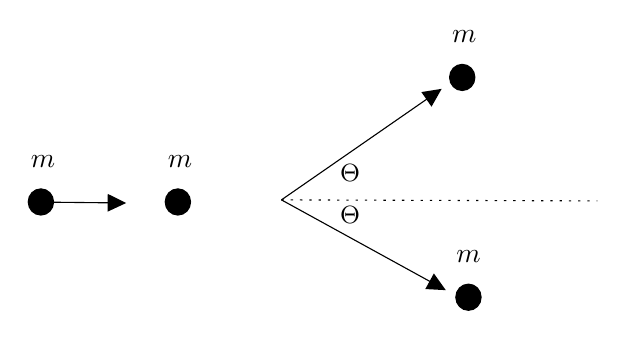
\begin{tikzpicture}[x=0.75pt,y=0.75pt,yscale=-1,xscale=1]
%uncomment if require: \path (0,300); %set diagram left start at 0, and has height of 300

%Flowchart: Connector [id:dp5958808506829039] 
\draw  [fill={rgb, 255:red, 0; green, 0; blue, 0 }  ,fill opacity=1 ] (88,130.7) .. controls (88,127.22) and (90.73,124.4) .. (94.1,124.4) .. controls (97.47,124.4) and (100.2,127.22) .. (100.2,130.7) .. controls (100.2,134.18) and (97.47,137) .. (94.1,137) .. controls (90.73,137) and (88,134.18) .. (88,130.7) -- cycle ;
%Straight Lines [id:da774514922768274] 
\draw    (88,130.7) -- (132.2,131.17) ;
\draw [shift={(135.2,131.2)}, rotate = 180.61] [fill={rgb, 255:red, 0; green, 0; blue, 0 }  ][line width=0.08]  [draw opacity=0] (8.93,-4.29) -- (0,0) -- (8.93,4.29) -- cycle    ;
%Flowchart: Connector [id:dp9275966313304485] 
\draw  [fill={rgb, 255:red, 0; green, 0; blue, 0 }  ,fill opacity=1 ] (154,130.7) .. controls (154,127.22) and (156.73,124.4) .. (160.1,124.4) .. controls (163.47,124.4) and (166.2,127.22) .. (166.2,130.7) .. controls (166.2,134.18) and (163.47,137) .. (160.1,137) .. controls (156.73,137) and (154,134.18) .. (154,130.7) -- cycle ;
%Flowchart: Connector [id:dp2448775352971747] 
\draw  [fill={rgb, 255:red, 0; green, 0; blue, 0 }  ,fill opacity=1 ] (291,70.7) .. controls (291,67.22) and (293.73,64.4) .. (297.1,64.4) .. controls (300.47,64.4) and (303.2,67.22) .. (303.2,70.7) .. controls (303.2,74.18) and (300.47,77) .. (297.1,77) .. controls (293.73,77) and (291,74.18) .. (291,70.7) -- cycle ;
%Flowchart: Connector [id:dp020775563565975985] 
\draw  [fill={rgb, 255:red, 0; green, 0; blue, 0 }  ,fill opacity=1 ] (294,176.6) .. controls (294,173.12) and (296.73,170.3) .. (300.1,170.3) .. controls (303.47,170.3) and (306.2,173.12) .. (306.2,176.6) .. controls (306.2,180.08) and (303.47,182.9) .. (300.1,182.9) .. controls (296.73,182.9) and (294,180.08) .. (294,176.6) -- cycle ;
%Straight Lines [id:da6654713491922019] 
\draw    (210,129.7) -- (284.73,77.91) ;
\draw [shift={(287.2,76.2)}, rotate = 145.28] [fill={rgb, 255:red, 0; green, 0; blue, 0 }  ][line width=0.08]  [draw opacity=0] (8.93,-4.29) -- (0,0) -- (8.93,4.29) -- cycle    ;
%Straight Lines [id:da4816667891850749] 
\draw    (210,129.7) -- (286.57,171.76) ;
\draw [shift={(289.2,173.2)}, rotate = 208.78] [fill={rgb, 255:red, 0; green, 0; blue, 0 }  ][line width=0.08]  [draw opacity=0] (8.93,-4.29) -- (0,0) -- (8.93,4.29) -- cycle    ;
%Straight Lines [id:da5822391697912397] 
\draw  [dash pattern={on 0.84pt off 2.51pt}]  (210,129.7) -- (362.2,130.2) ;

% Text Node
\draw (88,107) node [anchor=north west][inner sep=0.75pt]   [align=left] {$\displaystyle m$};
% Text Node
\draw (154,107) node [anchor=north west][inner sep=0.75pt]   [align=left] {$\displaystyle m$};
% Text Node
\draw (291,47) node [anchor=north west][inner sep=0.75pt]   [align=left] {$\displaystyle m$};
% Text Node
\draw (293,153) node [anchor=north west][inner sep=0.75pt]   [align=left] {$\displaystyle m$};
% Text Node
\draw (237,111.4) node [anchor=north west][inner sep=0.75pt]  [font=\small]  {$\Theta $};
% Text Node
\draw (237,131.4) node [anchor=north west][inner sep=0.75pt]  [font=\small]  {$\Theta $};


\end{tikzpicture}

\end{center}
\caption{The same two billiard balls colliding as in lecture 9, but now with the incoming billiard moving with relativistic velocity. }\label{fig:billiards}
\end{figure}
\subsubsection*{Example 1: Relativistic Billiards}

In the lecture on Newtonian dynamics, we showed that the preferred angle of two billiard balls colliding after collision was $90^\circ$. Now, let us reconsider this problem for relativistic billiards (see Fig.~\ref{fig:billiards}). Again, we have two billiards, each of mass $m$. One of them is at rest, while the other is moving with velocity $v_1$ to the right (on course for a collision). Let us find the angle $\Theta$ after the collision in terms of the incoming energy $E$ of one of the particles and the mass $m$ of the particles. 

First, we write down the relevant energy-momentum 4-vectors before 
\be
P_1 &=& (E,p,0,0)\\
P_2 &=& (m,0,0,0),
\ee
and after the collision:
\be
P_1' &=& (E',p'\cos\Theta, p'\sin \Theta,0)\\
P_2' &=& (E',p'\cos\Theta, -p'\sin \Theta, 0 ). 
\ee
We use that $p'=\sqrt{E'^2-m^2}$ and $p = \sqrt{E^2-m^2}$, and $E' = (E+m)/2$ (energy conservation) while $p = 2p'\cos \Theta$ (conservation of momentum in $x$ direction). Then also $p' \sin \Theta  = \frac{p}{2} \tan \Theta $. We thus write
\be
P'_{1,2} = \left( \frac{E+m}{2}, \frac{p}{2}, \pm \frac{p}{2}\tan \Theta, 0\right).
\ee
Now using that $P^2 = m^2$, we write
\be
P_1 \cdot P_1 =P_2 \cdot P_2= m^2 = \left(\frac{E+m}{2}\right)^2 -\left(\frac{p}{2}\right)^2 (1 + \tan^2 \Theta).
\ee
We multiply both sides by $4$ and use $p^2 = E^2 - m^2$ and realize that 
\be 1+ \tan^2 \Theta &=& 1 + \frac{\sin^2 \Theta}{ \cos^2 \Theta} 
= \frac{\cos^2 \Theta}{\cos^2 \Theta} + \frac{\sin^2 \Theta}{ \cos^2 \Theta} \nonumber  \\ &=& \frac{\cos^2 \Theta + \sin^2 \Theta}{\cos^2\Theta}= \frac{1}{\cos^2\Theta},
\ee
we find
\be
4 m^2 = (E^2 + m^2) -(E^2 - m^2)\frac{1}{\cos^2 \Theta}. 
\ee
Solving for $\cos \Theta$
\be
\cos^2 \Theta = \frac{E^2 -m^2}{E^2+2Em-3m^2} = \frac{E+m}{E+3m}. 
\ee
If we take the relativistic limit, i.e., when $E\gg m$, we find $\cos \Theta \simeq 1$, or $\Theta\rightarrow 0$. So the particles scatter almost directly forward. 

Instead, if we consider the non-relativistic limit, we have $E\simeq m$ (rest energy) and we find that $\cos \Theta \simeq 1/\sqrt{2}$, or $\Theta  = 45^\circ$, and indeed the billiards would make a right angle as derived previously. 

Note that we never wrote any of the velocities, i.e., we never considered the expressions $\gamma m$ for the energy and $\gamma m v$ for the momentum. We only relied on conservation and $E^2 - p^2 = m^2$. 






\begin{figure}  
\centering

\begin{tikzpicture}[x=0.75pt,y=0.75pt,yscale=-1,xscale=1]
%uncomment if require: \path (0,300); %set diagram left start at 0, and has height of 300

%Flowchart: Connector [id:dp32135042087645227] 
\draw  [fill={rgb, 255:red, 0; green, 0; blue, 0 }  ,fill opacity=1 ] (108,150.7) .. controls (108,147.22) and (110.73,144.4) .. (114.1,144.4) .. controls (117.47,144.4) and (120.2,147.22) .. (120.2,150.7) .. controls (120.2,154.18) and (117.47,157) .. (114.1,157) .. controls (110.73,157) and (108,154.18) .. (108,150.7) -- cycle ;
%Straight Lines [id:da8319602961813328] 
\draw    (108,150.7) -- (152.2,151.17) ;
\draw [shift={(155.2,151.2)}, rotate = 180.61] [fill={rgb, 255:red, 0; green, 0; blue, 0 }  ][line width=0.08]  [draw opacity=0] (8.93,-4.29) -- (0,0) -- (8.93,4.29) -- cycle    ;
%Flowchart: Connector [id:dp2282471821148817] 
\draw  [fill={rgb, 255:red, 0; green, 0; blue, 0 }  ,fill opacity=1 ] (225.2,74) .. controls (225.2,71.68) and (226.99,69.8) .. (229.2,69.8) .. controls (231.41,69.8) and (233.2,71.68) .. (233.2,74) .. controls (233.2,76.32) and (231.41,78.2) .. (229.2,78.2) .. controls (226.99,78.2) and (225.2,76.32) .. (225.2,74) -- cycle ;
%Straight Lines [id:da2195966103738317] 
\draw    (230,149.7) -- (229.23,82.8) ;
\draw [shift={(229.2,79.8)}, rotate = 89.34] [fill={rgb, 255:red, 0; green, 0; blue, 0 }  ][line width=0.08]  [draw opacity=0] (8.93,-4.29) -- (0,0) -- (8.93,4.29) -- cycle    ;
%Straight Lines [id:da9815670362591361] 
\draw    (230,149.7) -- (306.57,191.76) ;
\draw [shift={(309.2,193.2)}, rotate = 208.78] [fill={rgb, 255:red, 0; green, 0; blue, 0 }  ][line width=0.08]  [draw opacity=0] (8.93,-4.29) -- (0,0) -- (8.93,4.29) -- cycle    ;
%Straight Lines [id:da896082722611167] 
\draw  [dash pattern={on 0.84pt off 2.51pt}]  (230,149.7) -- (382.2,150.2) ;
%Flowchart: Connector [id:dp7431155814311812] 
\draw  [fill={rgb, 255:red, 0; green, 0; blue, 0 }  ,fill opacity=1 ] (312.2,198) .. controls (312.2,195.68) and (313.99,193.8) .. (316.2,193.8) .. controls (318.41,193.8) and (320.2,195.68) .. (320.2,198) .. controls (320.2,200.32) and (318.41,202.2) .. (316.2,202.2) .. controls (313.99,202.2) and (312.2,200.32) .. (312.2,198) -- cycle ;
%Shape: Right Angle [id:dp4327473202947082] 
\draw   (253.2,143.8) -- (235.31,143.92) -- (235.2,127.8) ;

% Text Node
\draw (107,125) node [anchor=north west][inner sep=0.75pt]   [align=left] {$\displaystyle M$};
% Text Node
\draw (222,50) node [anchor=north west][inner sep=0.75pt]   [align=left] {$\displaystyle m$};
% Text Node
\draw (313,173) node [anchor=north west][inner sep=0.75pt]   [align=left] {$\displaystyle m$};
% Text Node
\draw (257,151.4) node [anchor=north west][inner sep=0.75pt]  [font=\small]  {$\Theta $};
% Text Node
\draw (109,162) node [anchor=north west][inner sep=0.75pt]   [align=left] {$\displaystyle E$};


\end{tikzpicture}
\caption{Mass $M$ decays into two small masses $m$, one of which moves straight up in the diagram and one moves away with an angle w.r.t. the horizontal axis.}\label{fig:decay}
\end{figure}


\subsubsection*{Example 2: Decay at an angle}
We do not really have a classical example of this.  We have a particle of mass $M$ and energy $E$ moving to the right. This particle decays into two new particles (see fig.~\ref{fig:decay}). One will be moving vertically up, while the other one will move with a tilted direction downward, making an angle $\Theta$ with the $x$ axis. What are the energies of the created particles? 

Before the decay, we have 
\be
P = (E,p,0,0),
\ee
and after the decay, we have 
\be
P_1 &=& (E_1,0,p_1,0), \nonumber \\
P_2 &=& (E_2,p_2 \cos \Theta,-p_2 \sin \Theta,0).
\ee
Conservation of momentum in the $x$ direction implies $p = p_2 \cos \Theta \rightarrow p_2\sin \Theta = p \tan \Theta$ since $p_y = 0$ before the decay:
\be
P_1 &=& (E_1,0,p \tan \Theta,0), \nonumber \\
P_2 &=& (E_2,p ,-p \tan \Theta,0). 
\ee
Conservation of energy gives $E = E_1 + E_2$ and using $m^2  = E^2 -|{\bf p}|^2$, we find 
\be
E = \sqrt{p^2\tan^2 \Theta +m^2}+\sqrt{p^2(1+\tan^2 \Theta) +m^2}.
\ee
To obtain an expression for the energies, we write:
\be
E = E_1 + E_2 \rightarrow E_1 = E-E_2,
\ee
and 
\be
p = p_2\cos \Theta.
\ee
We have 
\be
0 = p_1-p_2 \sin \Theta\rightarrow p_1= p_2 \sin \Theta
\ee
When we square the last two equations we get
\be
p^2 &=& p_2^2\cos^2 \Theta \nonumber, \\
p_1^2 &=& p_2^2 \sin^2 \Theta.
\ee
Combining these, tells us that $p_1^2 + p^2 = p_2^2 \rightarrow p^2 = p_2^2 -p_1^2$. We also square the equation for energy conservation to obtain $E_1^2 = E^2+E_2^2 - 2 EE_2$. Next, we use $m^2 = E_2^2-p_2^2 = E_1^2-p_1^2$, to find 
\be
E_1^2 = E^2 + E_1^2-p_1^2+p_2^2-2EE_2.
\ee
Then using $p^2 = p_2^2 -p_1^2$ we rewrite
\be
E_1^2 = E^2 + E_1^2+p^2-2EE_2 \rightarrow E_2 = \frac{E^2 +p^2}{2E},
\ee
and 
\be
E_1 = E-E_2 = \frac{M^2}{2E}.
\ee
Suppose the masses of the decay products are given by $m$. For what value of $\Theta$ would you get the maximum value of $m$? $E_1^2 = p^2 \tan^2\Theta + m^2 \rightarrow (E^2-M^2) \tan^2 \Theta + m^2 = (M^2/2E)^2$. Since the $\tan^2\Theta$ term is non-negative, the maximum mass is found when $\tan \Theta = 0$, or when $\Theta = 0^\circ$. For that angle, $m = M^2/2E$. The maximum mass is reached when the minimal amount of momentum is generated in the $y$ direction (otherwise, you will lose more mass). We can write $m = M^2/2E = M^2/(2\gamma M)$ or $2m = \gamma^{-1}M$. For $v\ll c$, $\gamma^{-1} = 1$, and hence we have the Newtonian results $2m  = M$. In all other cases, you lose mass (since the sum of the masses will be less than $2m$ as $\gamma^{-1}\leq 1$). Note that this is for $\Theta = 0^\circ$. For angles away from this, more mass will be lost. 

Now the inverse is also true. If you smash two particles against each other with high velocities, you can generate a new particle with $M\gg 2m$. This is exactly what particle colliders rely on.

In many cases, there is a much quicker way of solving these problems if we use 4-vectors. We can write 
\be
P = P_1 + P_2 \rightarrow P_2 = P -P_1.
\ee
We can square this:
\be
(P-P_1)\cdot(P-P_1) &=& P\cdot P - 2 P \cdot P_1 + P_1 \cdot P_1\nonumber \\
&=&P_2 \cdot P_2.
\ee
Now we use $P^2 = M^2$, $P_{1,2}^2 = m^2$, and the fact that in the cross term $P\cdot P_1$ only the temporal component $P_0$ survives:
\be
M^2 - 2E E_1+m^2 = m^2 \rightarrow E_1 = \frac{M^2}{2E}
\ee
and 
\be
E_2 = E-E_1 = (2E^2 -M^2)/2E.
\ee
So we have obtained the same result in only a couple of lines. Note that the effectiveness becomes even more apparent when you have more particles, which would scatter in more dimensions. Then the line-by-line projection will become very involved, but this way would remain tractable. 

\section{Particle Physics Units}\label{sec:PPU}
Particle physics is a branch of physics where special relativity applies (more specifically, quantum field theory, the intercept of quantum physics and special relativity). We already showed that colliding particles allow you to generate particles with masses that exceed the sum of the two colliding particles. 

What is the typical size of the rest energy of, e.g., a proton (used in the collider in CERN)? $m_p = 1.67\times 10^{-27}$ kg. The rest energy in SI is thus:
\be
E_p = m_p c^2 \simeq 1.5 \times 10^{-10}{\rm J}.
\ee
This number is very small. For that reason, particle physicists (all variants, e.g., astro-particle physicists, particle cosmologists) prefer to use``eV" or electron Volts as a base unit of energy. An electron volt is the energy equivalent of the change in energy of an electron when it passes through a potential difference of one volt. The charge of the electron is $1.602\times 10^{-19}$ C and one volt is defined as $1\; {\rm V} = 1\;{\rm J/C}$. Hence, from dimensional analysis, we thus have 
\be
1\;{\rm eV} = (1.602 \times 10^{-19})\;{\rm C} (1\; {\rm J/C}) = 1.602 \times 10^{-19}\; {\rm J}.
\ee
Using this as a base unit, we then find that $E_p = 938\times 10^6$ eV, or about 1 GeV (Giga electron-volt). The electron, which is about 2000 times lighter compared to the proton, has a rest energy of $E_e\simeq 0.5 $ MeV, so half a Mega electron-volt. 

While the units are energy units, in many cases particle physicists tend to talk about the masses of particles in the same way, i.e., the mass of a proton is 1 GeV. What is implicitly assumed is that $c=1$, and hence energy and mass have the same dimensions. 

To go back to SI, we can use
\be
1\;{\rm MeV}/c^2 = 1.783\times10^{-30}\;{\rm kg}. 
\ee

Now consider two protons colliding head-on. Our goal is to generate a Higgs particle in the process. Assume the protons have identical but opposite momentum, while the Higgs has no momentum ($v_H = 0$). We now know that $M_H \simeq  125$ GeV from experiment. Before the collision, the energy of the protons is $E_p = \gamma m_p$. This has to be equated with $2E_p = M_H$. Given the mass of the proton $m_p \simeq 1$ GeV we write 
\be
\gamma = \frac{M_H}{2 m_p} \simeq 62.5. 
\ee
This is the required Lorentz factor. We can find the required velocity to get such a high Lorentz factor:
\be
v = \sqrt{1-(62.5)^{-2}} \simeq 0.9998,
\ee
which is very close to the speed of light. 
\ifshowboardquestion
\section*{Board Question}
\begin{tcolorbox}[colback=blue!5!white]
A particle of mass $M$ is initially at rest and decays into two identical particles of mass $m$.
\begin{enumerate}
    \item Use momentum conservation to determine the directions of the two daughter particles.
    \boardanswer{The initial momentum is zero, so the daughter momenta must be equal in magnitude and opposite in direction.}
    \item Use energy conservation to find the energy of each daughter particle.
    \boardanswer{By symmetry each daughter carries half the initial rest energy: $E_1=E_2=M/2$ in units with $c=1$.}
    \item Find the speed of each daughter particle in terms of $M$ and $m$.
    \boardanswer{$\gamma m=M/2$, so $\gamma=M/(2m)$ and $v=\sqrt{1-1/\gamma^2}=\sqrt{1-4m^2/M^2}$.}
    \item What condition on $M$ and $m$ is required for the decay to be possible?
    \boardanswer{We need $M\geq2m$. Equality means the daughters are produced at rest; for motion, $M>2m$.}
\end{enumerate}
\end{tcolorbox}
\fi

\end{document}
